% description de l'algo de lehot
L'algorithme de {\em couverture} que nous proposons est une am\'elioration de celui de {\em Lehot}.
Ainsi, nous pr\'esentons bri\`evement le principe de l'algorithme de couverture en cliques de {\em Lehot} \cite{decompositionEnCliquesParArcs}. 
\newline
Soient $H$ et $G$ deux graphes. Nous supposons que $H$ est le line-graphe de $G$ ($H=L(G)$).
Le but de cet algorithme est d'identifier le graphe racine $L^{-1}(H)$ de $H$.
L'algorithme va construire $G$  au fur et \`a mesure en identifiant les cliques dans $H$. 
Les ar\^etes et les sommets de $H$ et $G$ peuvent avoir au cours de l'ex\'ecution plusieurs \'etats :
%''----------- sommets de H et G 
\begin{itemize}
	\item Sommet ``bien-d\'efini'' : un sommet d\'ecouvert de $G$ tel que la clique correspondante dans $H$ a \'et\'e trouv\'ee et identifi\'ee.
	\item Sommet ``\`a moiti\'e-nomm\'e'' :  un sommet de $H$ tel que  l'ar\^ete correspondante dans $G$ a une extr\'emit\'e  ``bien-d\'efinie''. 
	\item Sommet ``pleinement-nomm\'e'' : un sommet de $H$ tel que l'ar\^ete correspondante dans $G$  a des extr\'emit\'es ``bien-d\'efinies''.
	\item Sommet ``basique'' : un sommet de $H$ est une ar\^ete de $G$. Ces sommets sont not\'es $x-y$ dans $H$ avec $x$ et $y$ des sommets d\'ecouverts de $G$.
	\item Sommet ``partag\'e'' : sommet de $H$ partageant une ar\^ete avec des sommets ``basiques'' adjacents. Ce sommet est une extr\'emit\'e commune entre des ar\^etes de $G$ incidentes. 
\end{itemize}
%''----------- sommets de H et G 


L'id\'ee de cet algorithme est de d\'eterminer une couverture de corr\'elation de $H$ en d\'etectant, selon $3$ cas \cite{decompositionEnCliquesParArcs} dans $H$, 
les sommets partag\'es adjacents \`a un sommet ``basique'' qui forment une clique.
Nous illustrons le fonctionnement de l'algorithme avec l'exemple suivant illustr\'e par la figure \ref{deroulementAlgorithmeLehotRechercheSommetsPartages}.
L'algorithme s\'electionne deux sommets ``basiques''  $1-2, 2-3$ et  l'ensemble $X$ des sommets adjacents aux sommets ``basiques''.
Si $X = \emptyset$ alors il n'existe pas de sommet partag\'e dans  $G$ et les sommets $1-2, 2-3$ sont \'etiquet\'es ``\`a moiti\'e-nomm\'e'' (figure \ref{deroulementAlgorithmeLehotRechercheSommetsPartages}(a)).
Si $X=\{x\}$ alors le sommet $x$ est un sommet partag\'e dans  $H$ si $x = 2-4$ car le triangle $\{x, 1-2, 2-3\}$ est impair. Dans le cas o\`u $x = 1-3$, le  triangle $\{x, 1-2, 2-3\}$ est pair et
aucun sommet d\'ecouvert dans $G$ n'est incident aux sommets du triangle $\{x, 1-2, 2-3\}$ (figure \ref{deroulementAlgorithmeLehotRechercheSommetsPartages}(b)). 
Le sommet $x$ dans $H$ est \'etiquet\'e ``pleinement-nomm\'e'' et les autres sommets $1-2, 2-3$ dans $H$ sont \'etiquet\'es ``\`a moiti\'e-nomm\'e''.
Si $X=\{x,y\}$, il n'existe  aucun sommet partag\'e dans  $H$ si $x$ et $y$ sont adjacents dans $H$. Dans le cas o\`u  ils ne sont pas adjacents alors ils forment deux triangles avec $1-2, 2-3$. Si $x=2-4$ et $y=1-3$ alors le triangle $\{2-4,1-2, 2-3\}$ est impair et $x$ est le sommet partag\'e dans $H$
(figure \ref{deroulementAlgorithmeLehotRechercheSommetsPartages}(c)).
Enfin pour $|X| = |\{a,b,c, \cdots\}| = 3$, le sommet $b$ dans $H$ est \'etiquet\'e sommet partag\'e si $a$ est adjacent \`a $b$ sinon le sommet $a$ devient le sommet partag\'e.
La derni\`ere \'etape s\'electionne al\'eatoirement un sommet ``\`a moiti\'e-nomm\'e'' dans $H$ qui est adjacent \`a un sommet  ``pleinement-nomm\'e'' dans $H$. Si ce sommet n'est pas d\'ej\`a couvert par une clique alors il est ``pleinement-nomm\'e'' et il est un sommet partag\'e dans $H$. 
\`A la fin de cette \'etape, tous les sommets sont \'etiquet\'es \`a ``pleinement-nomm\'e"  dans $H$ et ils deviennent des sommets partag\'es dans $H$.
\newline
L'algorithme s'ex\'ecute  en $O(m)+m'$ avec $m$  le nombre d'ar\^etes dans $G$ et $m'$ le nombre d'ar\^etes dans $L(G)$. Il retourne la liste de cliques d\'ecouvertes dans $H$ dans laquelle chaque clique correspond  \`a un sommet de $G$. Cette liste de cliques est appel\'ee {\em couverture de corr\'elation} (${\cal CC}$).
Malheureusement, si $H$ n'est pas un line-graphe alors il ne retourne pas de couverture partielle.

\subsubsection{Description de l'algorithme de couverture}
Nous proposons  l'algorithme de {\em couverture} (voir algorithme \ref{algo:couverture}) en lien avec celui de {\em Lehot} qui couvre  autant que possible les sommets du graphe de corr\'elation  $G_c$ par une ou deux cliques.
Notre algorithme retourne la {\em couverture de corr\'elation} (${\cal CC}$) de $G_c$ si la matrice d'adjacence de $G_c$ ne contient aucune case erron\'ee sinon il renvoie une {\em couverture de corr\'elation partielle} de $G_c$.
\newline
%% ---- figure etapes de decouverte de l'algo de lehot
\begin{figure}[htb!]
	\centering
	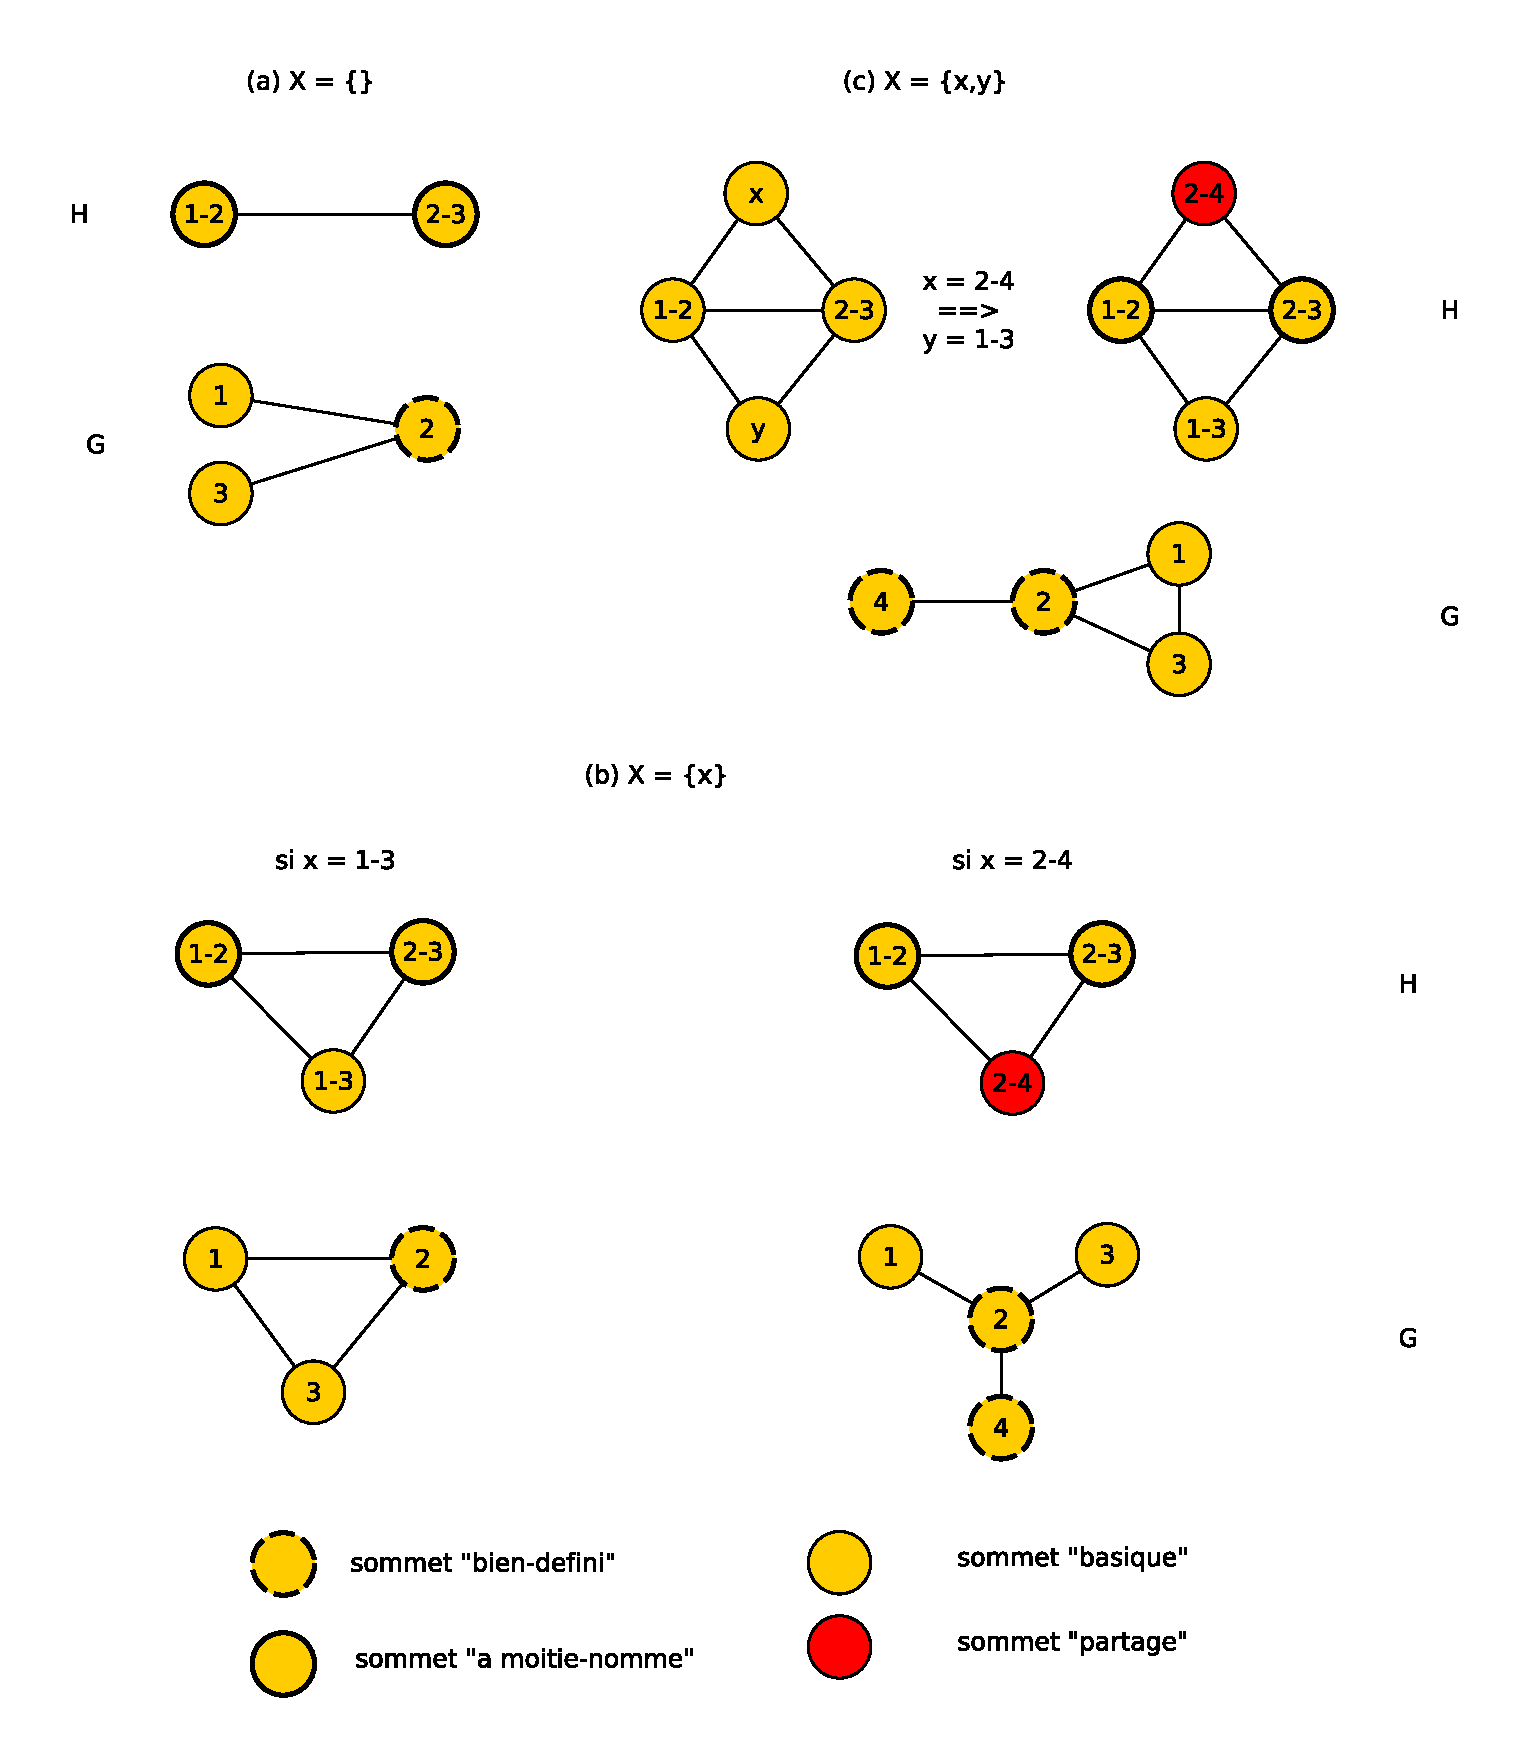
\includegraphics[scale=0.50]{deroulementAlgorithmeLehot.eps}\vspace{-0.5em}
	\caption{ Identification des sommets partag\'es dans le graphe $H$ et nommage des sommets de $G$. }\vspace{-0.5em}
	\label{deroulementAlgorithmeLehotRechercheSommetsPartages}
\end{figure}
%% ---- figure etapes de decouverte de l'algo de lehot
\FloatBarrier

Soient $G_c = (V,E)$ un graphe de corr\'elation et $Cliq(v)$ l'\'etat de chaque sommet $v$ de   $G_c$.
L'algorithme de {\em couverture} va construire une couverture de corr\'elation ${\cal CC}(G_c)$ de $G_c$ en ajoutant des cliques d\'ecouvertes dans ${\cal CC}(G_c)$.  
Une clique est un ensemble de sommets qui induit un sous-graphe complet. 
Si un sommet appartient \`a une clique alors il est couvert par cette clique. 
De m\^eme, si deux sommets $u$ et $v$ appartiennent \`a une m\^eme clique, alors la clique couvre l'ar\^ete $[x,y]$.
Initialement ${\cal CC}(G_c)$ est vide et chaque sommet de $v \in V$ a un \'etat $Cliq(v)=0$. 
\newline
\`A chaque \'etape de l'algorithme, chaque sommet $v$ a $5$ \'etats possibles :
\begin{itemize}
	\item $Cliq(v)=0$ : le sommet $v$ n'est couvert par aucune clique. Il correspond \`a un sommet ``basique'' dans l'algorithme de {\em Lehot}.
	\item $Cliq(v)=1$ : le sommet $v$ est couvert par une clique ou deux cliques. Dans le cas o\`u il est couvert par deux cliques, l'intersection de ces cliques donne le sommet $v$. Ce sommet est \'etiquet\'e ``pleinement-nomm\'e" dans l'algorithme de {\em Lehot}.
	\item $Cliq(v) = 2$ : le sommet $v$ est couvert par une clique et peut \^etre couvert par une seconde clique. Ce sommet est ``bien-nomm\'e" dans l'algorithme de {\em Lehot}.
	\item $Cliq(v) = 3$ : le sommet $v$ est un sommet ambigu. L'algorithme doit identifier la clique \`a laquelle il appartient pour qu'elle devienne un sommet partag\'e dans l'algorithme de {\em Lehot}.
	\item $Cliq(v) = -1$ :  le sommet $v$ est couvert par plus de deux cliques. Il est contenu dans l'ensemble $\cal C$ et doit \^etre corrig\'e par l'algorithme de correction.
\end{itemize}

Nous choisissons un sommet $v$ de degr\'e minimum qui n'appartient \`a aucune clique ou qui est un sommet ambigu. 
S'il existe une partition coh\'erente (voir d\'efinition \ref{cliquesCoherentes}) de ce sommet et de son voisinage $\{v\} \cup \Gamma_{G_c}(v)$ en deux cliques $C_1, C_2$, alors ces deux cliques sont contenues dans la couverture de corr\'elation ${\cal CC}(G_c)$ en cours de construction. Les sommets $v$ et $u$ (avec $u \in  \Gamma_{G_c}(v)$), appartenant \`a $C_1$ ou $C_2$, ont leur \'etat modifi\'e \`a chaque \'etape de l'algorithme de la mani\`ere suivante :
\begin{itemize}
\item $Cliq(v) = 1$ si son \'etat pr\'ec\'edent est \'egal \`a $0$ et la clique $C_2$ est vide. 
\item $Cliq(v) = 3$ si son \'etat pr\'ec\'edent est \'egal \`a $0$ et la clique $C_2$ est non vide. 
\item $Cliq(v) = 2$ si son \'etat pr\'ec\'edent est diff\'erent de $0$.
\item $Cliq(u) = 1$ si son \'etat pr\'ec\'edent est \'egal \`a $0$ et l'ensemble des ar\^etes incidentes \`a $u$ est vide.
\item $Cliq(u) = 2$ si son \'etat pr\'ec\'edent est \'egal \`a $3$ et l'ensemble des ar\^etes incidentes \`a $u$ est vide.
\item $Cliq(u) = 3$ si son \'etat pr\'ec\'edent est \'egal \`a $0$ et l'ensemble des ar\^etes incidentes \`a $u$ est non vide.
\item $Cliq(u) = -1$ si son \'etat pr\'ec\'edent est \'egal \`a $3$ et l'ensemble des ar\^etes incidentes \`a $u$ est non vide.
\end{itemize} 
Dans le cas o\`u il n'existe aucune partition coh\'erente (voir d\'efinition \ref{cliquesCoherentes}) au sommet $v$, son \'etat est \`a $Cliq(v)=-1$.
\newline
%\vspace{-1.5cm}
  %% ---- figure etapes de decouverte de l'algo de lehot
\begin{figure}[htb!]
	\centering
	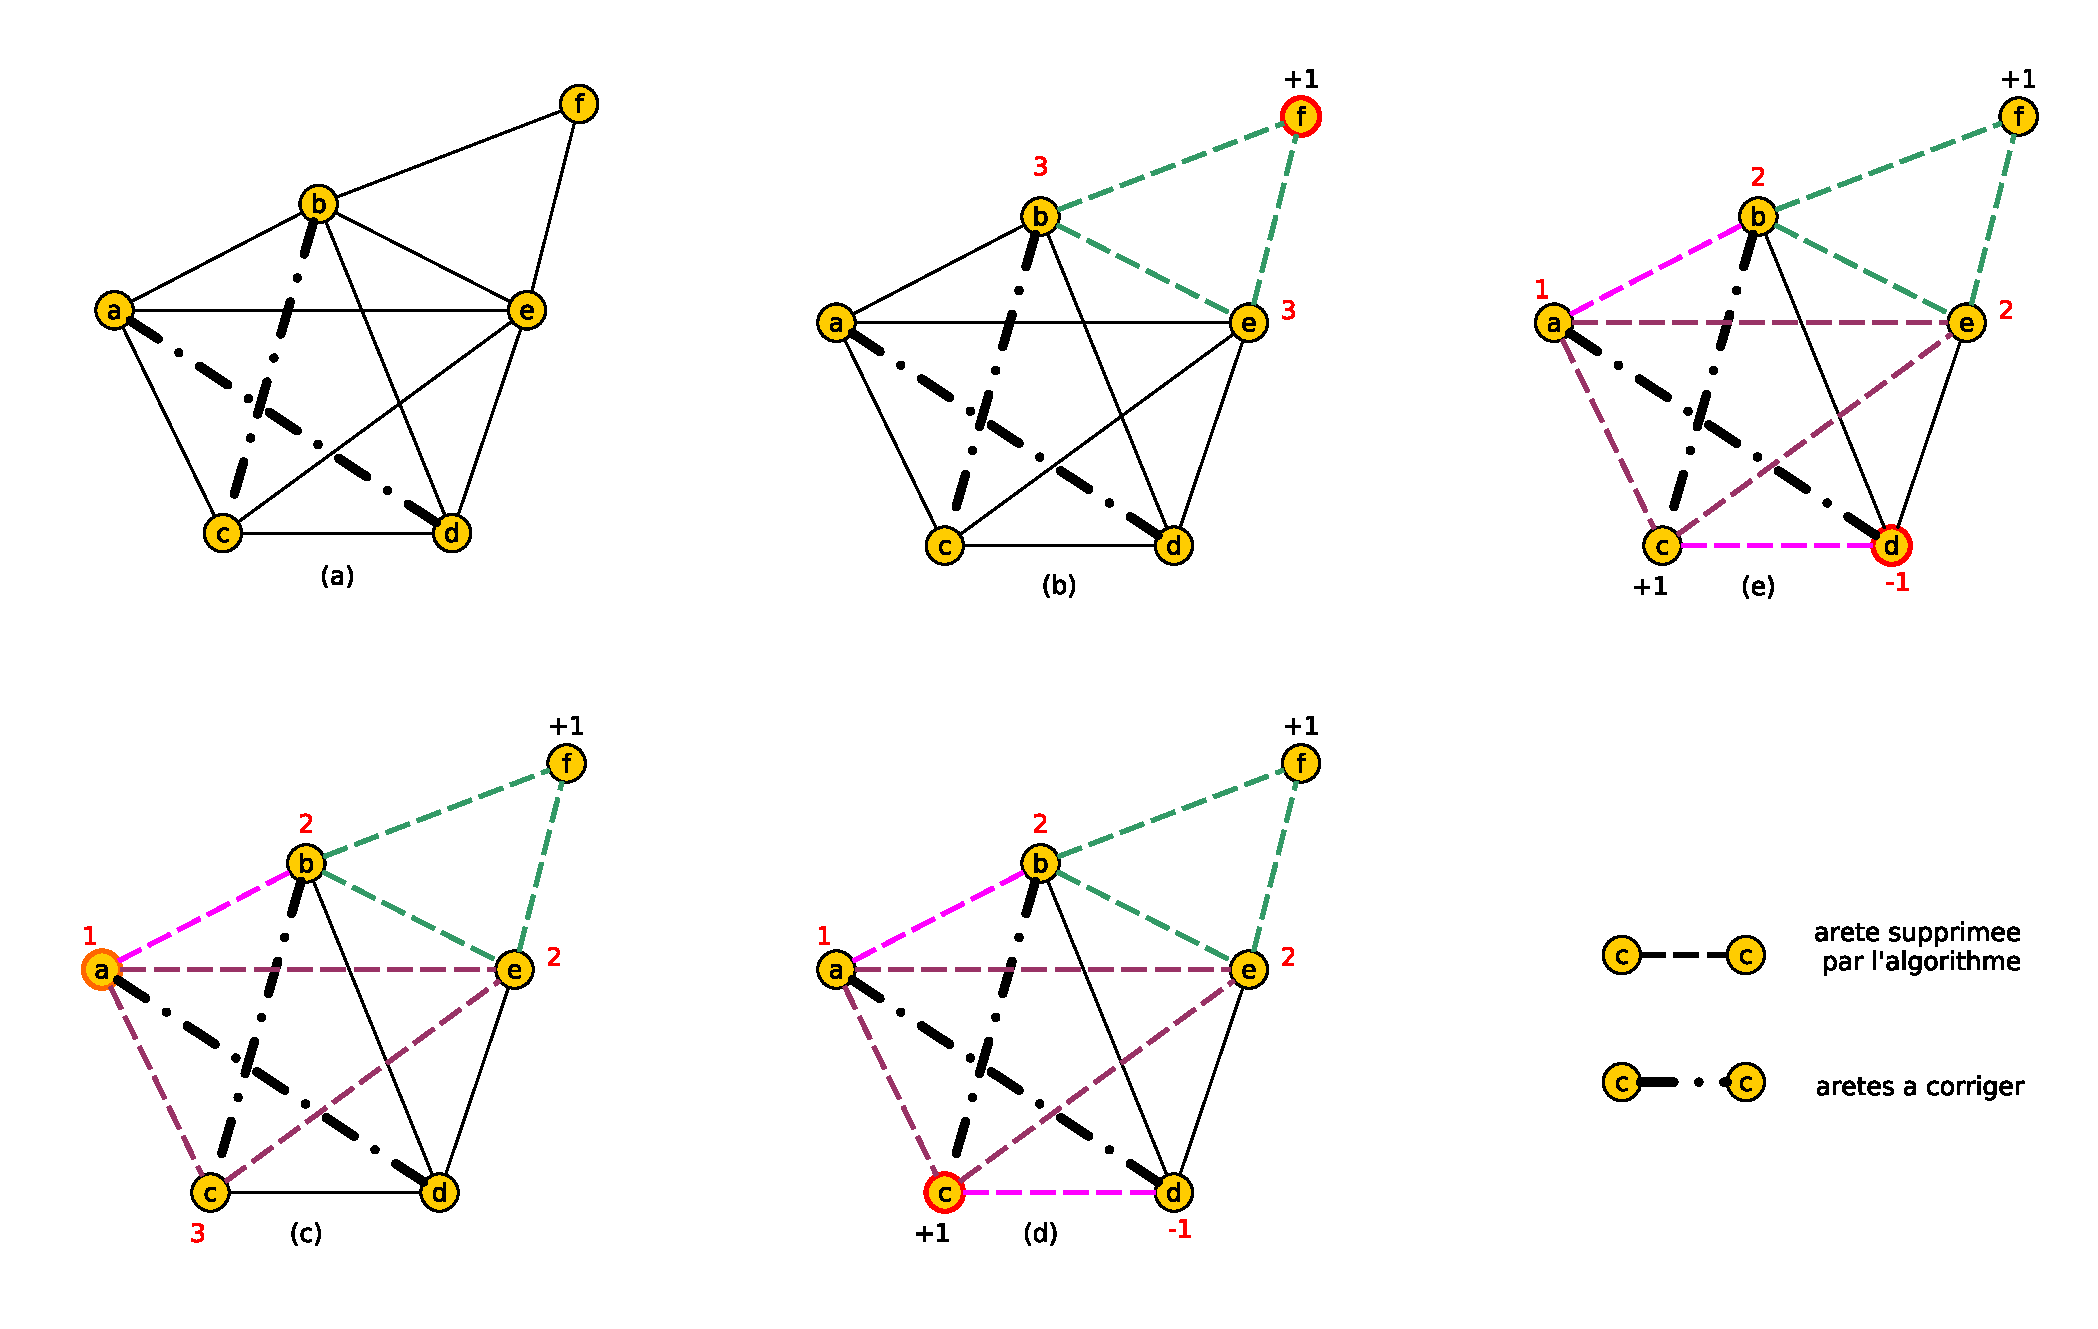
\includegraphics[width=500pt, height= 300pt]{exempleAlgorithmeCouverture.eps}\vspace{-0.5em}
	\caption{ Les diff\'erentes \'etapes de la couverture en cliques du graphe $G$. Les ar\^etes de m\^eme couleur appartiennent \`a la m\^eme clique.  Les ar\^etes $(b,c)$ et $(a,d)$ sont supprim\'ees du graphe avant l'ex\'ecution de l'algorithme de {\em couverture}.  }\vspace{-0.5em}
	\label{exempleAlgorithmeCouverture}
\end{figure}
%% ---- figure etapes de decouverte de l'algo de lehot
\FloatBarrier
%% description de l'algo
L'algorithme de recherche de couverture de corr\'elation ${\cal CC}(G_c)$ (voir algorithme \ref{algo:couverture})  consid\`ere, tant qu'il en existe, un sommet $v$ dont les ar\^etes incidentes sont couvertes par une seule clique. 
Il affecte \`a ce sommet l'\'etat $Cliq(v) = 1$, sauvegarde cette clique dans ${\cal CC}(G_c)$ puis supprime ces ar\^etes incidentes dans le graphe $G_c$. Les voisins de ce sommet passent \`a l'\'etat $2$.
\newline
Si au cours de l'ex\'ecution un tel sommet $v$ n'existe pas alors l'algorithme de {\em couverture} consid\`ere un sommet $u$ dont son voisinage peut \^etre couvert par deux cliques et qui n'a pas \'et\'e pr\'ec\'edemment couvert par une clique de ${\cal CC}(G_c)$. 
Si cette partition en deux cliques est unique, l'algorithme affecte $Cliq(u) = 1$ \`a ce sommet et supprime les ar\^etes. 
Dans le cas o\`u ce sommet appartient \`a un des cas de la figure \ref{configurationAmbiguite} (cas d'un sommet encadr\'e), nous avons montr\'e que ces graphes sont les seuls line-graphes pour lesquels deux partitions possibles existent. 
Nous utilisons la fonction de d\'ecision  $Verif-correl$  (section \ref{VerifCorrel}) pour lever l'ambigu\"{i}t\'e.
\newline
Un \'etat est affect\'e aux autres sommets $v$ de la clique couvrant $v$ selon l'un des trois cas. 
Dans le premier cas, l'\'etat actuel appartient \`a $Cliq(v) \in \{2,3\}$ si les sommets $v$ ont des ar\^etes incidentes non encore couvertes par une clique et l'\'etat pr\'ec\'edent est $Cliq(v) \in \{ 3,0\}$. 
Dans le second cas, $Cliq(v) = 1$ est attribu\'e aux sommets $v$ si l'ensemble des ar\^etes incidentes est vide. 
Enfin, dans le dernier cas, l'algorithme  affecte $Cliq(v) = -1$ \`a ces sommets si leur \'etat pr\'ec\'edent est  $Cliq(v) \in \{2,3\}$ et leurs ar\^etes incidentes ne forment pas une clique.
\newline
\`A la fin  de l'ex\'ecution de cet algorithme, tous les sommets $v$ dont l'\'etat courant est $Cliq(v) = -1$  n'ont pas \'et\'e couverts. 
Ces sommets appartiennent \`a l'ensemble $\cal C$ des sommets \`a corriger par l'algorithme de correction.
\newline

 La figure \ref{exempleAlgorithmeCouverture} d\'etaille l'algorithme de {\em couverture} (algorithme \ref{algo:couverture})  sur un graphe $G=(V,E)$  dans lequel nous avons supprim\'e deux ar\^etes. L'objectif de la suppression d'ar\^etes dans la figure \ref{exempleAlgorithmeCouverture}(a) est d'obtenir des sommets \`a corriger \`a la fin de la couverture.
 Nous s\'electionnons le sommet $f$ car il est de degr\'e minimum. 
 Il forme une clique avec son voisinage alors la clique $\{f,b,e\}$ est ajout\'ee \`a l'ensemble  ${\cal CC}(G)$ puis les ar\^etes $(f,b), (b,e), (f,e)$ sont supprim\'ees de $E$. 
 L'\'etat de $f$ est $Cliq(f) = 1$ et les sommets $b$ et $e$ ont $Cliq(b) = Cliq(e) = 3$ (voir figure \ref{exempleAlgorithmeCouverture}(c)). 
 \newline
 Le second sommet trait\'e est $a$ car son \'etat est $Cliq(a) = 0$. Il existe deux partitions coh\'erentes $\{a,b\}$ et $\{a,e,c\}$ au voisinage de $a$. Ces deux partitions sont ajout\'ees \`a    ${\cal CC}(G)$ et les ar\^etes de ces cliques sont supprim\'ees de $E$. L'algorithme attribue 
 \begin{itemize}
\item  Au sommet $a$, l'\'etat $Cliq(a) = 1$,
\item Aux sommets $b$ et $e$, les \'etats $Cliq(b) = Cliq(e) = 2$ car leur \'etat pr\'ed\'ecent \'etait $Cliq(b) = Cliq(e) = 3$ et ces sommets ont encore un voisin,
\item Au sommet $c$, l'\'etat $Cliq(b) = 3$.
 \end{itemize}
 On traite les autres sommets ($c$) de la m\^eme mani\`ere jusqu'\`a ce qu'on s\'electionne le sommet $d$.
 Ce sommet a deux partitions $\{d,b\}$ et $\{d,e\}$ non coh\'erentes (voir d\'efinition \ref{cliquesCoherentes}) parce que la fonction $Verif-correl$ (section \ref{VerifCorrel}) appliqu\'ee \`a ces partitions retourne 0. 
 Ce sommet est donc \`a corriger ${\cal C} = \{d\}$ (voir figure \ref{exempleAlgorithmeCouverture}(e)).
\newline

Si le graphe $G_c=(V_c, E_c)$ est un graphe de corr\'elation alors l'algorithme de couverture en d\'etermine la couverture de corr\'elation ${\cal CC}(G_c)$.
En effet, si $G_c$ est un line-graphe, par r\'ecurrence sur l'ensemble des sommets et \`a chaque \'etape, il existe un sommet non encore couvert qui :
\begin{itemize}
\item Soit est couvert par une clique appartenant \`a ${\cal CC}(G_c)$ et son voisinage restant peut \^etre convert par une nouvelle clique.
\item Soit n'est couvert par aucune clique de  ${\cal CC}(G_c)$ et son voisinage restant peut \^etre couvert par une ou deux nouvelles cliques.
\item Soit est dans une ambigu\"{i}t\'e alors on a recours \`a la fonction $Verif-correl$ (section \ref{VerifCorrel}) pour d\'eterminer les bonnes partitions de ce sommet.
\end{itemize}

\subsubsection{Complexit\'e de l'algorithme de couverture}

Si $G_c$ est un line-graphe, le sommet choisi $u$ (s'il existe) \`a la ligne $4$ de l'algorithme \ref{algo:couverture}  est \`a l'\'etat $Cliq(u) = 0$ et le sommet $u$ n'est pas un sommet ambigu. Dans le cas contraire, il est \`a l'\'etat $Cliq(u) = 3$.
Chaque s\'election de sommets conduit \`a  une unique et correcte partition et aussi \`a une seule couverture de corr\'elation. 
Nous montrons par induction sur l'ensemble des sommets qu'\`a chaque \'etape de l'algorithme \ref{algo:couverture}, il y a un sommet :
\begin{itemize}
	\item Non couvert par aucune clique et certains de ses voisins peuvent \^etre couverts par $1$ ou $2$ nouvelles cliques ($Cliq(u) = 0$, voir graphe $(b)$ de la figure \ref{exempleAlgorithmeCouverture}).
	\item Couvert par une clique d\'ej\`a dans la couverture de corr\'elation ${\cal CC}$ et ses voisins non couverts peuvent \^etre couverts par une nouvelle clique  ($Cliq(u) = 3$, voir graphe $(c)$ de la figure \ref{exempleAlgorithmeCouverture}).
\end{itemize} 
L'algorithme de couverture d\'etermine la couverture de corr\'elation si $G_c$ est v\'eritablement un line-graphe.

En revanche, si le graphe $G_c$ n'est pas un line-graphe alors, \`a certaines \'etapes de l'ex\'ecution, deux diff\'erents m\'ethodes de couvrir le sommet choisi par des cliques peuvent se pr\'esenter. Dans certains cas, nous choisissons al\'eatoirement  une des m\'ethodes (cela peut avoir un impact sur l'algorithme de correction). 
Notons que nous r\'ealisons les m\^emes op\'erations si le graphe $G_c$ est non connexe, m\^eme si des composantes connexes sont isomorphes aux graphes de la figure  \ref{neufSousGraphesInterditDesLineGraphes}. 
Le line-graphe obtenu est toujours un graphe connexe.
\newline

Concernant la complexit\'e, d\'eterminer si un sommet $u$ de $G_c$ est couvert par $1$ ou $2$ cliques a une complexit\'e de $O(\Delta(G_c)^2)$ (en d\'eterminant si le nombre chromatique du graphe compl\'ementaire est $1$ ou $2$). 
Alors la complexit\'e de l'algorithme de couverture est dans le pire des cas $O(n \times \Delta(G_c)^2)$ avec $n$ le nombre de sommets.  
Rappelons que l'algorithme de Lehot \cite{decompositionEnCliquesParArcs} a une complexit\'e de $O(n \times \Delta(G_c))$. Cependant, il ne fournit pas de couverture de corr\'elation partielle lorsque  $G_c$ n'est pas un line-graphe.
\newline

{\bf Conclusion} : si le graphe $G_c$ est un line-graphe, tous ses sommets $v$ sont labellis\'es \`a $Cliq(v) = 1$ et l'algorithme  de {\em couverture} trouve une partition du voisinage d'un sommet en une ou deux cliques de fa\c con unique (voir les lemmes pr\'ec\'edents). 
Une fois ce sommet et ses ar\^etes incidentes supprim\'ees, le graphe restant est toujours un line-graphe, et la propri\'et\'e se propage.
%Donc, si $G_c$ est un line-graphe, cet algorithme en trouvera toujours la couverture de corr\'elation unique.
Ainsi $G_c$ qui poss\`ede des sommets $v$ aux \'etats $Cliq(v) = -1$ n'est pas un line-graphe. Nous proposons l'algorithme de correction qui retourne le line-graphe le plus proche de $G_c$.


%---------------------------- algorithme de couverture ---------------------------------------------------------------------
\begin{algorithm}
\algsetup{indent=2em}
\caption{Couverture}
\label{algo:couverture}
\begin{algorithmic}[1]
\IF{$G_c$ est isomorphe \`a un graphe double (voir figure \ref{graphe2Couverture})}
	\STATE{le traiter avec $Verif-correl$ $(^1)$}
\ELSE
	\WHILE {il existe un sommet $u$ t.q $Cliq(u) \in \{0,3\}$}
		\STATE{ choisir un sommet $u$ de degr\'e minimum}
		\IF{ $\{u\} \cup \Gamma_{G_c}(u)$ peut \^etre couvert par deux cliques $C_1$ et $C_2$ coh\'erentes, \\ ~~~~~~$C_1$ maximale et $C_2 = \emptyset$ si $Cliq(u)=3$ $(^2)$ }
			\IF{$Cliq(u) = 0$ et $C_2 \neq \emptyset$}
				\STATE{ $Cliq(u)= 3$ }
			\ELSE
				\IF{$Cliq(u) = 0$ et $C_2 =  \emptyset$}
					\STATE{$Cliq(u) = 1$}
				\ELSE
					\STATE{$Cliq(u) = 2$}
				\ENDIF
			\ENDIF
			\STATE{ $\epsilon_u = E(G_c[C_1]) \cup E(G_c[C_2])$ }
			\FOR{$w \in \Gamma_{G_c}(u)$}
				\STATE{ $\alpha(w) = card\{[w,x] \in E - \epsilon_u\}$}
				\IF{$\alpha_w > 0$}
					\IF{ $Cliq(w) = 0$ }
						\STATE{$Cliq(w) = 3$}
					\ELSE
						\IF{$Cliq(w) = 3$}
							\STATE{$Cliq(w) = -1$}
						\ENDIF	
					\ENDIF
				\ELSE
					\IF{$Cliq(w) = 0$}
						\STATE{$Cliq(w) = 1$}
					\ELSE
						\IF{$Cliq(w) = 3$}
							\STATE{$Cliq(w) = 2$}
						\ENDIF
					\ENDIF
				\ENDIF
			\ENDFOR
			\STATE{$E = E - \epsilon_{u}$}
		\ELSE
			\STATE{$Cliq(u) = -1$}
		\ENDIF
	\ENDWHILE
\ENDIF
\end{algorithmic}
\end{algorithm}
%
%\begin{algorithm}[!ht]
%\label{algo:couverture}
%\caption{couverture}
%%\begin{algorithmic}[1]
%\noindent DEBUT\\
%\noindent 1. {\bf Si} $G_c$ est isomorphe \`a un graphe double (voir figure \ref{graphe2Couverture} ), {\bf alors} le traiter avec Verif-correl$(^1)$ \\
%~~\indent {\bf Sinon} \\
%~2. \indent {\bf Tant que} il existe un sommet $u$ t.q $Cliq(u) \in \{0,3\}$\\ 
%       	\indent~~~~~~{\bf Faire}\\
%~3.	       	\indent~~~~~~~~choisir $u$ de degr\'e minimum\\
%~4.       	\indent~~~~~~~~{\bf Si} $\{u\} \cup \Gamma_{G_c}(u)$ peut \^etre couvert par deux cliques $C_1$ et $C_2$ coh\'erentes,\\
%		\indent~~~~~~~~~~~~~~$C_1$ maximale et $C_2 = \emptyset$ si $Cliq(u)=3$ $(^2)$\\
%	       	\indent~~~~~~~~~~~~{\bf alors}\\
%~5.	       	\indent~~~~~~~~~~~~~~{\bf Si } $Cliq(u) = 0$ et $C_2\neq \emptyset$ {\bf Alors} $Cliq = 3$ \\
%~6.		\indent~~~~~~~~~~~~~~{\bf Sinon Si} $Cliq = 0$ et $C_2 =  \emptyset$ {\bf Alors} $Cliq(u) = 1$\\
%~7.		\indent~~~~~~~~~~~~~~~~~~~~~~~{\bf Sinon} $Cliq(u) = 2$ 	\\
%~8.		\indent~~~~~~~~~~~~~~~~~~~~~~~{\bf FinSi}\\      	
%~9.		\indent~~~~~~~~~~~~~~{\bf FinSi}\\
%~10.		\indent ~~~~~~~~~~~~~$\epsilon_u = E(G_c[C_1]) \cup E(G_c[C_2])$\\
%~11.		\indent ~~~~~~~~~~~~~{\bf Pour tout} $w \in \Gamma_{G_c}(u)$ {\bf Faire} \\
%~12.		\indent~~~~~~~~~~~~~~~~$\alpha(w) = card\{[w,x] \in E - \epsilon_u\}$\\
%~13.		\indent~~~~~~~~~~~~~~~~{\bf Si} $\alpha_w > 0$ {\bf Alors}\\
%~14.		\indent~~~~~~~~~~~~~~~~~~{\bf Si} $Cliq(w) = 0$ {\bf Alors} $Cliq(w) =3$\\
%~15.		\indent~~~~~~~~~~~~~~~~~~{\bf Sinon Si} $Cliq(w) = 3$ {\bf Alors} $Cliq(w) =-1$\\
%~16.		\indent~~~~~~~~~~~~~~~~~~{\bf FinSi} \\
%~17.		\indent~~~~~~~~~~~~~~~~{\bf Sinon Si} $Cliq(w) = 0$ {\bf Alors} $Cliq(w) =1$\\
%~18. 	\indent~~~~~~~~~~~~~~~~~~~~~~~~~{\bf Sinon Si} $Cliq(w) = 3$ {\bf Alors} $Cliq(w) = 2$ \\
%~19. 	\indent~~~~~~~~~~~~~~~~~~~~~~~~~{\bf FinSi} \\
%~20.		\indent ~~~~~~~~~~~~~{\bf FinPourTout}\\
%~21.		\indent ~~~~~~~~~~~~~$E = E - \epsilon_u$\\
%~22.		\indent            ~~~~~~~{\bf Sinon} $Cliq(u) = -1$\\
%	       	\indent~~~~~~~~~~~~{\bf FinSi}\\
%%       	\indent~~~~~~
%~23. \indent {\bf FinTant que}\\
%~24. \noindent {\bf Fin Si}\\
%\noindent FIN\\
%%\end{algorithmic}
%\end{algorithm}
%---------------------------- algorithme de couverture ---------------------------------------------------------------------

\FloatBarrier
$^1$ : chaque graphe de la figure \ref{graphe2Couverture} admet deux couvertures de corr\'elation, souvent isomorphes, mais une seule de ces couvertures de corr\'elation peut correspondre au DAG du r\'eseau \'electrique sous-jacent. Dans ce cas, on utilise la fonction $Verif-correl$ afin de d\'eterminer la couverture de corr\'elation la plus probable.
\newline

 $^2$ :  le sommet $u$ choisi (s'il existe) ne sera pas prioritairement un sommet tel que $Cliq(u) = 0$ et $u$ est un point d'ambigu\"{i}t\'e. Si lors d'une \'etape, seul un tel choix est possible et qu'il n'y a aucun sommet $u$ tel que $Cliq(u) = -1$, c'est que chaque sommet du graphe initial $G_c$ est un point d'ambigu\"{i}t\'e.
 Dans ce cas, $G_c$ est une union de composantes connexes isomorphes \`a un des graphes de la figure  \ref{graphe2Couverture}.
Dans ce cas, n'importe quel choix conduit \`a une couverture de corr\'elation correcte.
